\section{分布与推前}
\label{sec:pspace-distributions}

随机变量是样本空间上的函数，可是多数问题只关心它的取值落在哪里、各处概率多大，并不关心是哪个样本点产生了这个取值。第~\ref{chap:random-variables}章把这种“取值的规律”称为分布，并只对区间及其有限并计算过它。现在把分布定义为取值空间上的一个完整的概率测度。

\paragraph{分布的定义}
随机对象$X$把每个样本点$\omega$送到$E$中的点$X(\omega)$。把$\omega$所带的概率质量随之搬过去，$E$中集合$B$所收到的质量，就是被送进$B$的那些样本点的质量之和，即$\mathbb{P}(X^{-1}(B))$。

\begin{definition}[分布]
\label{def:pspace-distribution}
设$X$是取值于$(E,\mathcal{E})$的随机对象。称
\begin{equation}
  P_X(B)=\mathbb{P}\bigl(X^{-1}(B)\bigr)=\mathbb{P}(X\in B),\qquad B\in\mathcal{E},
  \label{eq:pspace-distribution}
\end{equation}
为$X$的分布。$P_X$是$\mathbb{P}$在$X$下的推前测度，也记作$\mathbb{P}\circ X^{-1}$。
\end{definition}

$P_X$是$(E,\mathcal{E})$上的概率测度。总质量$P_X(E)=\mathbb{P}(\Omega)=1$；若$B_1,B_2,\dots$两两不交，它们的原像也两两不交，并且原像之并等于并集的原像，于是由$\mathbb{P}$的可数可加性，
\[
  P_X\Bigl(\bigcup_kB_k\Bigr)=\mathbb{P}\Bigl(\bigcup_kX^{-1}(B_k)\Bigr)=\sum_k\mathbb{P}\bigl(X^{-1}(B_k)\bigr)=\sum_kP_X(B_k).
\]
推前测度的一般理论，包括映射下的密度公式，可参考\BookChapterRef{chap:pushforward-measures}{卷四第9章“推前测度”}。

有了$P_X$，关于$X$取值的问题都可以在$(E,\mathcal{E},P_X)$上回答，不必再回到$\Omega$。第~\ref{chap:random-variables}章说“取值集合可以当作新的样本空间”，现在有了准确的含义：$(E,\mathcal{E},P_X)$本身就是一个概率空间。

\paragraph{用原像计算分布}
在木棍模型$\Omega=[0,1)$上定义$X(\omega)=-\ln(1-\omega)$。$X$连续且严格递增，从$0$增加到$+\infty$，因而是随机变量。对$x\geq0$，$X>x$等价于$\omega>1-\mathrm{e}^{-x}$，所以
\[
  \mathbb{P}(X>x)=\lambda\bigl((1-\mathrm{e}^{-x},1)\bigr)=\mathrm{e}^{-x}.
\]
这正是$\operatorname{Exp}(1)$的右尾概率：均匀的质量经过$X$的搬运，变成了指数分布。

用同一个原像规则可以算任何区间的概率。取$B=(1,2]$，它的原像是$\omega$轴上的区间$(1-\mathrm{e}^{-1},1-\mathrm{e}^{-2}]$，于是
\[
  P_X\bigl((1,2]\bigr)=(1-\mathrm{e}^{-2})-(1-\mathrm{e}^{-1})=\mathrm{e}^{-1}-\mathrm{e}^{-2}\approx0.2325 .
\]
图~\ref{fig:pspace-pushforward-exp}(a)把这个原像画了出来：纵轴上的$B$经曲线反射到横轴，得到长约$0.865-0.632$的区间。图~\ref{fig:pspace-pushforward-exp}(b)是同一概率在取值空间上的样子，即指数密度在$(1,2]$上的面积。

\begin{BookInlineFigure}
  \centering
  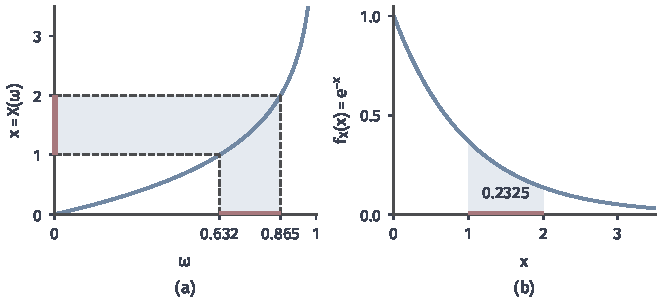
\includegraphics[width=112mm]{figures/07-probability/02-measure-theoretic-probability/matplotlib/pspace-pushforward-exp/figure.pdf}
  \caption{用原像计算推前分布。(a)蓝线是$x=X(\omega)=-\ln(1-\omega)$，纵轴上的红色线段是$B=(1,2]$，它的原像是横轴上的红色线段$(0.632,0.865]$，长度$\mathrm{e}^{-1}-\mathrm{e}^{-2}$；(b)取值空间上的分布，浅蓝面积是$P_X((1,2])\approx0.2325$。}
  \label{fig:pspace-pushforward-exp}
\end{BookInlineFigure}

对实值随机变量，分布函数$F_X(x)=P_X((-\infty,x])$就是式~\eqref{eq:pspace-cdf}对$P=P_X$的特例。由定理~\ref{thm:pspace-cdf-measure}，$F_X$确定了整个$P_X$：两个随机变量的分布函数相同，它们落在任何Borel集中的概率都相同。第~\ref{chap:random-variables}章只能从分布函数读出区间的概率，这一缺口现在补上了。

\paragraph{变换后的分布}
对随机对象再作可测变换$Y=g(X)$，$Y$的分布可以只用$X$的分布算出。对$B\in\mathcal{E}'$，$\{Y\in B\}=\{X\in g^{-1}(B)\}$，所以
\begin{equation}
  P_{g(X)}(B)=P_X\bigl(g^{-1}(B)\bigr).
  \label{eq:pspace-transform-law}
\end{equation}
质量先由$X$从$\Omega$搬到$E$，再由$g$从$E$搬到$E'$，两次搬运的结果与一次搬运$g\circ X$相同。

截断的等待时间是一个例子。对指数变量$X$取$Y=\min\{X,2\}$，即$g(x)=\min\{x,2\}$。单点$\{2\}$的原像是$[2,\infty)$，由式~\eqref{eq:pspace-transform-law}，
\[
  P_Y(\{2\})=P_X\bigl([2,\infty)\bigr)=\mathrm{e}^{-2}\approx0.1353,
\]
而$y<2$时$P_Y((-\infty,y])=P_X((-\infty,y])$。$X$在$[2,\infty)$上的质量全部被搬到点$2$上，所以$Y$的分布在$2$处有一个原子，这就是第~\ref{chap:random-variables}章在分布函数上看到的跳跃。第~\ref{chap:random-variable-transformations}章的各种换元公式，都是在具体的$g$下计算式~\eqref{eq:pspace-transform-law}；离散、连续和混合的情形使用的是同一条原像规则。

\paragraph{任何分布函数都可以实现}
定理~\ref{thm:pspace-cdf-measure}在实轴上造出了以$F$为分布函数的概率测度。能否在某个概率空间上造出一个随机变量，使它的分布函数恰好是$F$？最直接的办法是把$(\mathbb{R},\mathcal{B}(\mathbb{R}),P)$本身当作样本空间，令$X(x)=x$。下面给出另一种构造，它只用木棍上的一个均匀点，后面构造独立序列时会反复用到。

对满足定理~\ref{thm:pspace-cdf-measure}条件的$F$，定义
\begin{equation}
  Q(u)=\inf\{x\in\mathbb{R}:\ F(x)\geq u\},\qquad 0<u<1 .
  \label{eq:pspace-quantile}
\end{equation}
这就是第~\ref{chap:random-variables}章的分位数函数。$0<u<1$保证集合$\{x:F(x)\geq u\}$非空（因为$F\to1$）且有下界（因为$F\to0$），所以$Q(u)$是有限实数。

\begin{lemma}[分位数函数的基本关系]
\label{lem:pspace-quantile}
对$0<u<1$与$x\in\mathbb{R}$，
\begin{equation}
  Q(u)\leq x\iff u\leq F(x).
  \label{eq:pspace-quantile-galois}
\end{equation}
\end{lemma}

\begin{proof}
若$u\leq F(x)$，则$x$属于集合$\{y:F(y)\geq u\}$，下确界不超过它，即$Q(u)\leq x$。

反过来，先证下确界本身属于这个集合。取集合中的一列点$y_n\downarrow Q(u)$，每个都满足$F(y_n)\geq u$。由右连续性，
\[
  F\bigl(Q(u)\bigr)=\lim_{n\to\infty}F(y_n)\geq u .
\]
于是若$Q(u)\leq x$，由$F$单调不减得$F(x)\geq F(Q(u))\geq u$。
\end{proof}

\begin{theorem}[分位数变换]
\label{thm:pspace-quantile-transform}
设$F$满足定理~\ref{thm:pspace-cdf-measure}的条件，$Q$由式~\eqref{eq:pspace-quantile}定义。在$\Omega=[0,1)$、$\mathcal{F}=\mathcal{B}([0,1))$、$\mathbb{P}=\lambda$上，令$X(\omega)=Q(\omega)$（$\omega>0$），$X(0)=0$。则$X$是随机变量，且$F_X=F$。
\end{theorem}

\begin{proof}
对$x\in\mathbb{R}$，由式~\eqref{eq:pspace-quantile-galois}，
\[
  \{\omega\in(0,1):X(\omega)\leq x\}=\{\omega\in(0,1):\omega\leq F(x)\}=(0,F(x)]\cap(0,1).
\]
$\{X\leq x\}$是这个区间与可能的单点$\{0\}$之并，是Borel集，由判别~\eqref{eq:pspace-rv-criterion}，$X$是随机变量。单点概率为零，所以
\[
  \mathbb{P}(X\leq x)=\lambda\bigl((0,F(x)]\cap(0,1)\bigr)=F(x),
\]
最后一步在$F(x)=1$时也成立，因为$(0,1)$的长度是$1$。
\end{proof}

用等待时间$W$走一遍。分布函数在$t\geq0$时为$F_W(t)=0.3+0.7(1-\mathrm{e}^{-t})$，在$0$处从$0$跳到$0.3$。由式~\eqref{eq:pspace-quantile}，$u\leq0.3$时最小的满足$F_W(x)\geq u$的点是$0$；$u>0.3$时解方程$F_W(x)=u$。于是
\begin{equation}
  Q_W(u)=\begin{cases}0,&0<u\leq0.3,\\ \ln\dfrac{0.7}{1-u},&0.3<u<1.\end{cases}
  \label{eq:pspace-waiting-quantile}
\end{equation}
取两个均匀随机数$u=0.2$与$u=0.37$，得到
\[
  Q_W(0.2)=0,\qquad Q_W(0.37)=\ln\frac{0.7}{0.63}=\ln\frac{10}{9}\approx0.1054 .
\]
第一个落在跳跃的高度范围内，对应“不用等”；第二个对应等待约$0.105$个单位时间。图~\ref{fig:pspace-quantile-transform}显示，分布函数在$0$处的跳跃，变成了分位数函数在$(0,0.3]$上的平台：长度为$0.3$的一段均匀质量全部被送到点$0$。

\begin{BookInlineFigure}
  \centering
  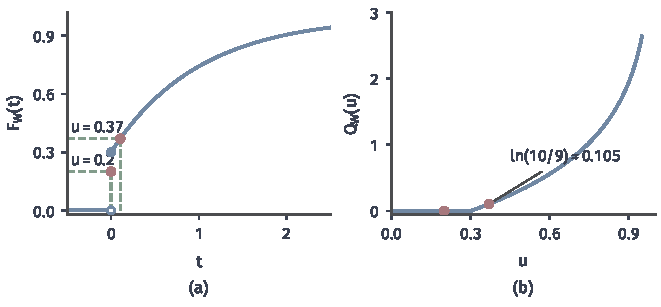
\includegraphics[width=112mm]{figures/07-probability/02-measure-theoretic-probability/matplotlib/pspace-quantile-transform/figure.pdf}
  \caption{用分位数变换从均匀随机数得到等待时间$W$。(a)蓝线是$F_W$；绿色虚线从高度$u$水平向右，碰到曲线（或跳跃的竖直段）后竖直向下，落点就是$Q_W(u)$；$u=0.2$落在跳跃内，得到$0$，$u=0.37$得到$\ln(10/9)$。(b)蓝线是$Q_W$，它在$(0,0.3]$上为$0$，红点是两个例子。}
  \label{fig:pspace-quantile-transform}
\end{BookInlineFigure}

定理~\ref{thm:pspace-quantile-transform}对Cantor分布同样适用，于是Cantor变量可以由一个均匀随机点得到。它也是从均匀随机数生成任意一维分布样本的基本方法，第~\ref{chap:sample-generation}章将讨论它的计算问题。

\paragraph{三种相等}
两个随机变量“相同”可以有三种不同强度的意思。设$X,Y$是同一概率空间上的随机变量。若对每个$\omega$都有$X(\omega)=Y(\omega)$，称它们处处相等；若$\mathbb{P}(X=Y)=1$，称它们几乎必然相等。第三种只比较分布，两个变量甚至可以定义在不同的概率空间上。

\begin{definition}[同分布]
\label{def:pspace-equal-in-law}
若随机对象$X$与$Y$取值于同一可测空间，且$P_X=P_Y$，则称$X$与$Y$同分布，记作
\begin{equation}
  X\overset{\mathrm{d}}{=}Y .
  \label{eq:pspace-equal-in-law}
\end{equation}
\end{definition}

三者依次减弱。处处相等时$\{X\neq Y\}=\varnothing$，所以处处相等蕴含几乎必然相等。若$X=Y$几乎必然成立，记$N=\{X\neq Y\}$，则对每个Borel集$B$，$\{X\in B\}$与$\{Y\in B\}$只在$N$中可能不同，它们的对称差包含于$N$，所以
\[
  \bigl\lvert P_X(B)-P_Y(B)\bigr\rvert\leq\mathbb{P}(N)=0,
\]
即$X\overset{\mathrm{d}}{=}Y$。

反方向都不成立。在木棍模型上取$U(\omega)=\omega$与$1-U$。对$u\in[0,1)$，
\[
  \mathbb{P}(1-U\leq u)=\mathbb{P}(U\geq1-u)=u,
\]
所以$1-U$也是均匀分布，$U\overset{\mathrm{d}}{=}1-U$。可是$U=1-U$只在$\omega=1/2$成立，$\mathbb{P}(U=1-U)=0$：两个同分布的变量几乎处处不相等，见图~\ref{fig:pspace-three-equalities}(a)。另一方面，把$U$在可数个点上改成$0$得到$U'$，例如在$\omega=k/8$（$k=1,\dots,7$）处，则$U'\neq U$只在一个零概率事件上发生，$U'=U$几乎必然成立，却不处处成立，见图~\ref{fig:pspace-three-equalities}(b)。

\begin{BookInlineFigure}
  \centering
  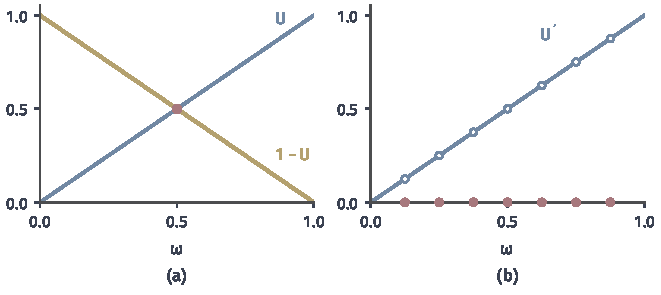
\includegraphics[width=112mm]{figures/07-probability/02-measure-theoretic-probability/matplotlib/pspace-three-equalities/figure.pdf}
  \caption{三种相等的区别，横轴是样本点$\omega\in[0,1)$。(a)蓝线$U(\omega)=\omega$与黄线$1-U$只在红点$\omega=1/2$处相等，二者却同为均匀分布；(b)$U'$在$\omega=k/8$处被改为$0$（红点），空心点是原来的值，其余位置与$U$相同，二者几乎必然相等。}
  \label{fig:pspace-three-equalities}
\end{BookInlineFigure}

这三种相等在实践中各有用处。一切只依赖分布的量，例如$\mathbb{P}(X>2)$、分位数以及第~\ref{sec:pspace-expectation}节将统一定义的期望，对同分布的变量都相同。几乎必然相等的变量还能在同一个样本点上互相替换，这在讨论多个变量的组合时是必需的。处处相等很少需要，因为零概率事件上的差别不影响任何概率。

\paragraph{边缘分布不能确定配对}
同分布的变量不能随意替换进组合中。仍取$X=U$与$X'=1-U$，二者同分布；再取$Y=U$，则
\[
  X+Y=2U,\qquad X'+Y=1 .
\]
前者均匀分布在$[0,2)$上，后者恒等于$1$。原因是$X+Y$的分布不只依赖$X$和$Y$各自的分布，还依赖它们在同一个样本点上怎样配对。

配对由联合分布描述。$(X,Y)$是取值于$\mathbb{R}^{2}$的随机向量，它的分布$P_{(X,Y)}$称为联合分布；$X$的分布是它在坐标投影$\pi_1(x,y)=x$下的推前，
\[
  P_X(B)=\mathbb{P}\bigl((X,Y)\in B\times\mathbb{R}\bigr)=P_{(X,Y)}\bigl(\pi_1^{-1}(B)\bigr).
\]
差$X-Y$是映射$(x,y)\mapsto x-y$下的推前，所以它的分布由联合分布确定，却不能由两个边缘分布确定。

下面三种配对的边缘都是$[0,1)$上的均匀分布：$(U,U)$、$(U,1-U)$，以及$(U,V)$，其中$V$是与$U$独立的另一个均匀变量（第~\ref{sec:pspace-independence}节在同一个概率空间上构造它）。记$D=X-Y$，三种配对下：
\begin{enumerate}
  \item $(U,U)$：$D\equiv0$，质量全部集中在原点；
  \item $(U,1-U)$：$D=2U-1$，均匀分布在$(-1,1)$上，密度为$1/2$；
  \item $(U,V)$：$D$的密度是$1-\lvert z\rvert$（$\lvert z\rvert<1$），即第~\ref{chap:random-variable-transformations}章算过的三角形密度。
\end{enumerate}
差的大小随配对变化很大。以$\mathbb{P}(\lvert D\rvert\leq0.1)$为例，三种配对依次是
\[
  1,\qquad \frac{0.2}{2}=0.1,\qquad 1-0.9^{2}=0.19 .
\]
第三个数是三角形密度在$[-0.1,0.1]$上的积分，等于$1$减去两侧两个直角三角形的面积$2\times\frac12\times0.9^{2}$。$D$的方差依次为$0$、$1/3$和$1/6$。

\begin{BookInlineFigure}
  \centering
  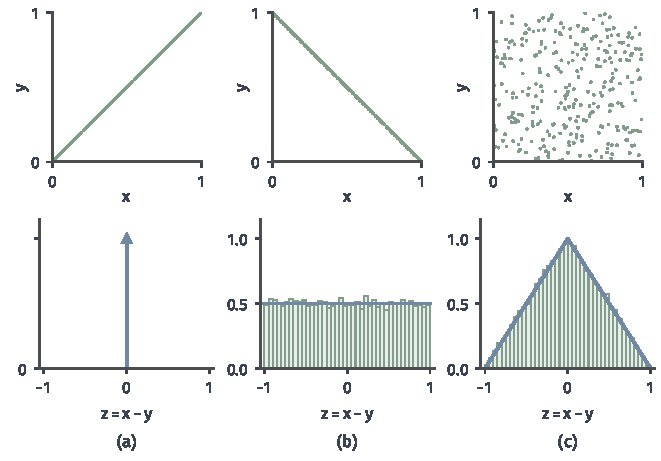
\includegraphics[width=112mm]{figures/07-probability/02-measure-theoretic-probability/matplotlib/pspace-couplings/figure.pdf}
  \caption{三种边缘相同的配对。上行是$300$对模拟样本（种子$9$）的散点：(a)$(U,U)$落在对角线上，(b)$(U,1-U)$落在反对角线上，(c)独立的$(U,V)$铺满正方形。下行是$D=X-Y$的分布：(a)全部质量在$0$（箭头表示单点质量$1$），(b)(c)中浅绿直方图来自$20000$对模拟样本，蓝线分别是均匀密度$1/2$与三角形密度$1-\lvert z\rvert$。}
  \label{fig:pspace-couplings}
\end{BookInlineFigure}

图~\ref{fig:pspace-couplings}的上行显示，三种配对的质量在平面上的位置完全不同，但向两条坐标轴的投影都是均匀分布。把同一组边缘分布配成联合分布的方式称为耦合，第~\ref{chap:optimal-transport}章研究怎样选择耦合使搬运代价最小。本章需要记住的是：随机变量本身、它的分布和多个变量的联合分布是三个不同层次的对象，从后者可以推出前者，反之不能。
